% questions.tex —— 1990 年·广东卷·文史类 · 题目内容片段（无答案）
% 由 tools/generate_projects.py 依来源总账自 1990/1990_广东_试题.md 生成，勿手改（改源 MD 后重跑）


\begin{gktip}
来源说明：固定源 7 页扫描件，印刷页 656–662。第一卷为选择 1–25，第二卷原以「一、二、三、四、五」编号，本库续编为 26–30 并在答案/解析中沿用该映射。卷内答案：第一卷有代号表；第二卷第一题列结果，第二题有详解，第三至五题只注「见理工农医类第二卷相应题解答」。

源疑点：第 11 题「侧面积为 $8\pi\ \mathrm{cm}^3$」按文意为 $\mathrm{cm}^2$，照录加注；

图形说明：第 18、28 题图依原页拓扑重绘，不按比例。

卷末原注：「1991 年，广东考生参加全国普通高等学校招生统一考试。」（照录，不属本卷题面内容。）
\end{gktip}

\begin{gktip}
卷面抬头：（文 史 类）　［试题］

卷面分「第 一 卷」「第 二 卷」两部分。第二卷大题卷面编号为一、二、三、四、五，其下再分小题；为便于与答案要点、解析逐题对应，本稿在答案与解析中续编为第 26—30 题。

页脚页码为 656—662（委托说明所记「636—642」与扫描页脚不符，此处以扫描页脚为准）。
\end{gktip}

\gkpart{第 一 卷}

\begin{question}
\gkti{1}如果 $0<\theta<\pi$，且 $\cos\theta=-\dfrac{\sqrt3}{2}$，那么 $\theta$ 等于（　）。

（A）$\dfrac{5\pi}{6}$；（B）$\dfrac{2\pi}{3}$；（C）$\dfrac{\pi}{3}$；（D）$\dfrac{\pi}{6}$。

\end{question}
\begin{question}
\gkti{2}函数 $f(x)=\sqrt{1+2x}+\sqrt{1-2x}$ 的定义域是（　）。

（A）$\left(-\infty,-\dfrac12\right]$；（B）$\left[\dfrac12,+\infty\right)$；（C）$\left[-\dfrac12,+\infty\right)$；（D）$\left[-\dfrac12,\dfrac12\right]$。

\end{question}
\begin{question}
\gkti{3}椭圆 $\dfrac{(x+1)^2}{16}+\dfrac{y^2}{25}=1$ 的离心率是（　）。

（A）$\dfrac35$；（B）$\dfrac34$；（C）$\dfrac{\sqrt{41}}{4}$；（D）$\dfrac{\sqrt{41}}{5}$。

\end{question}
\begin{question}
\gkti{4}双曲线 $\dfrac{y^2}{16}-\dfrac{x^2}{9}=1$ 的准线方程是（　）。

（A）$x=\pm\dfrac{16}{\sqrt7}$；（B）$y=\pm\dfrac{16}{\sqrt7}$；（C）$x=\pm\dfrac{16}{5}$；（D）$y=\pm\dfrac{16}{5}$。

\end{question}
\begin{question}
\gkti{5}$\cos^2 75^\circ+\cos^2 15^\circ+\cos 75^\circ\cdot\cos 15^\circ$ 的值等于（　）。

（A）$\dfrac{\sqrt6}{2}$；（B）$\dfrac54$；（C）$\dfrac32$；（D）$1+\dfrac{\sqrt3}{4}$。

\end{question}
\begin{question}
\gkti{6}如果 $\operatorname{tg}\theta=2$，那么 $\sin^2\theta+\sin\theta\cos\theta+\cos^2\theta=$（　）。

（A）$\dfrac73$；（B）$\dfrac75$；（C）$\dfrac54$；（D）$\dfrac53$。

\end{question}
\begin{question}
\gkti{7}如果 $ax+2y+1=0$ 与直线 $x+y-2=0$ 互相垂直，那么 $a$ 的值等于（　）。

（A）$-2$；（B）$-\dfrac23$；（C）$-\dfrac13$；（D）$1$。

\end{question}
\begin{question}
\gkti{8}如果直线 $l$ 是平面 $\alpha$ 的斜线，那么平面 $\alpha$ 内（　）。

（A）不存在与 $l$ 平行的直线；

（B）不存在与 $l$ 垂直的直线；

（C）与 $l$ 垂直的直线只有一条；

（D）与 $l$ 平行的直线有无穷多条。

\end{question}
\begin{question}
\gkti{9}某乒乓球队有 9 名队员，其中 2 名是种子选手，现要挑选 5 名队员参加比赛，种子选手都必须在内，那么不同的选法共有（　）。

（A）36 种；（B）35 种；（C）84 种；（D）126 种。

\end{question}
\begin{question}
\gkti{10}把 6 个不同的元素排成一排，那么不同的排法共有（　）。

（A）36 种；（B）120 种；（C）720 种；（D）1440 种。

\end{question}
\begin{question}
\gkti{11}一个圆台的母线长是上、下底面半径的等差中项，且侧面积为 $8\pi\ \mathrm{cm}^3$，母线长为（　）。

（A）4cm；（B）$2\sqrt2$ cm；（C）2 cm；（D）$\sqrt2$ cm。

（源疑点：卷面面积单位印作 $\mathrm{cm}^3$，按文意与卷内答案应为 $\mathrm{cm}^2$，此处照录原样。）

\end{question}
\begin{question}
\gkti{12}把复数 $1+i$ 对应的向量按顺时针方向旋转 $\dfrac{2\pi}{3}$，所得到向量对应的复数是（　）。

（A）$\dfrac{1-\sqrt3}{2}+\dfrac{-1+\sqrt3}{2}i$；

（B）$\dfrac{1-\sqrt3}{2}+\dfrac{-1-\sqrt3}{2}i$；

（C）$\dfrac{-1+\sqrt3}{2}+\dfrac{-1-\sqrt3}{2}i$；

（D）$\dfrac{-1+\sqrt3}{2}+\dfrac{1-\sqrt3}{2}i$。

\end{question}
\begin{question}
\gkti{13}一动点在圆 $x^2+y^2=1$ 上移动时，它与定点 $(3,0)$ 连线的中点的轨迹方程是（　）。

（A）$(x+3)^2+y^2=4$

（B）$(x-3)^2+y^2=1$

（C）$\left(x+\dfrac32\right)^2+y^2=\dfrac12$

（D）$(2x-3)^2+4y^2=1$

\end{question}
\begin{question}
\gkti{14}函数 $y=\dfrac{\sin x}{|\sin x|}+\dfrac{|\cos x|}{\cos x}+\dfrac{\operatorname{tg}x}{|\operatorname{tg}x|}+\dfrac{|\operatorname{ctg}x|}{\operatorname{ctg}x}$ 的值域是（　）。

（A）$\{-2,4\}$；（B）$\{-2,0,4\}$；（C）$\{-2,0,2,4\}$；（D）$\{-4,-2,0,4\}$。

\end{question}
\begin{question}
\gkti{15}复数 $(\sqrt3-i)^3$ 的三角形式是（　）。

（A）$8(\cos 90^\circ+i\sin 90^\circ)$；（B）$8(\cos 90^\circ-i\sin 90^\circ)$；

（C）$8(\cos 180^\circ+i\sin 180^\circ)$；（D）$8(\cos 270^\circ+i\sin 270^\circ)$。

\end{question}
\begin{question}
\gkti{16}如果函数 $y=(a+1)x-(a-2)x^2$ 是奇函数，那么 $a$ 的值等于（　）。

（A）$-2$；（B）$-1$；（C）$2$；（D）$1$。

\end{question}
\begin{question}
\gkti{17}函数 $y=(x+4)^2$ 在某区间上是减函数，这区间可以是（　）。

（A）$[+4,+\infty)$；（B）$(-\infty,+4]$；（C）$[-4,+\infty)$；（D）$(-\infty,-4]$。

\Needspace{0.4\textheight}
\end{question}
\begin{question}
\gkti{18}已知下图（图 4-6-6）是 $y=2\sin(\omega x+\phi)\left(|\phi|<\dfrac{\pi}{2}\right)$ 的图象，那么（　）。

（A）$\omega=2$，$\phi=-\dfrac{\pi}{6}$；（B）$\omega=2$，$\phi=\dfrac{\pi}{6}$；

（C）$\omega=\dfrac{10}{11}$，$\phi=\dfrac{\pi}{6}$；（D）$\omega=\dfrac{10}{11}$，$\phi=-\dfrac{\pi}{6}$。
\nopagebreak[4]
\begin{center}% 依固定扫描页重绘；仅示意曲线在 y 轴上的截距、零点位置与升降次序，不按比例。
% 卷面图 4-6-6：曲线过点 (0,1)，第二个正向零点标为 11π/12，该处曲线由下向上穿过 x 轴。
\begin{tikzpicture}[line width=.5pt,scale=1.05,font=\small]
  \draw[->] (-0.9,0)--(6.0,0) node[right] {$x$};
  \draw[->] (0,-2.7)--(0,2.8) node[above] {$y$};
  \node[below right=3pt] at (0,0) {$O$};
  \begin{scope}
    \clip (-0.85,-2.65) rectangle (5.95,2.75);
    \draw[domain=-0.45:5.55,samples=220,smooth] plot (\x,{2*sin(deg(2*\x+pi/6))});
  \end{scope}
  % y 轴截距 1。
  \draw (-0.07,1)--(0.07,1);
  \node[left] at (-0.12,1) {$1$};
  % 第二个正向零点，曲线在此由下向上穿过 x 轴。
  \draw (2.879,0.07)--(2.879,-0.07);
  \node[below left] at (2.80,-0.06) {$\dfrac{11\pi}{12}$};
\end{tikzpicture}
\end{center}
\nopagebreak[4]
\end{question}
\begin{question}
\gkti{19}如果 $x,y$ 是实数，那么“$xy=0$”是“$|x+y|=|x|+|y|$”的（　）。

（A）必要而且充分的条件；

（B）必要但不充分的条件；

（C）充分但不必要的条件；

（D）既不充分也不必要的条件。

\end{question}
\begin{question}
\gkti{20}如果直线 $y=ax+2$ 与直线 $y=3x-b$ 关于 $y=x$ 对称，那么（　）。

（A）$a=\dfrac13$，$b=-6$；（B）$a=\dfrac13$，$b=6$；（C）$a=3$，$b=-2$；（D）$a=3$，$b=6$。

\end{question}
\begin{question}
\gkti{21}如果抛物线 $y^2=ax$ 的准线方程为 $x=-1$，那么它的焦点坐标是（　）。

（A）$(1,0)$；（B）$(2,0)$；（C）$(3,0)$；（D）$(-1,0)$。

\end{question}
\begin{question}
\gkti{22}已知等比数列的公比是 2，且前 4 项之和等于 1，那么前 8 项之和等于（　）。

（A）21；（B）19；（C）17；（D）15。

\end{question}
\begin{question}
\gkti{23}函数 $y=\operatorname{tg}\dfrac{x}{2}-\dfrac{1}{\sin x}$ 的最小正周期是（　）。

（A）$\dfrac{\pi}{2}$；（B）$\pi$；（C）$\dfrac{3\pi}{2}$；（D）$2\pi$。

\end{question}
\begin{question}
\gkti{24}以一个三棱柱的顶点为顶点的四面体共有（　）。

（A）30 个；（B）18 个；（C）12 个；（D）6 个。

\end{question}
\begin{question}
\gkti{25}如果实数 $x,y$ 满足等式 $(x-2)^2+y^2=3$，那么 $\dfrac{y}{x}$ 的最大值是（　）。

（A）$\dfrac12$；（B）$\dfrac{\sqrt3}{3}$；（C）$\dfrac{\sqrt3}{2}$；（D）$\sqrt3$。

\end{question}
\gkpart{第 二 卷}

\begin{question}
\gkti{26}（本题满分 15 分）本题共有 5 小题，每小题都有用横线表示的空位，请把你认为合适的内容写在横线上方的空位里，每道小题满分 3 分。

（1） 已知 $\sin\alpha=\dfrac35$，$\alpha\in\left(\dfrac{\pi}{2},\pi\right)$，那么 $\sin\dfrac{\alpha}{2}$ 的值等于 \gkblank{}。

（2） $(x-1)-(x-1)^2+(x-1)^3-(x-1)^4$ 的展开式中，$x^2$ 的系数等于 \gkblank{}。

（3） $\lim\limits_{n\to\infty}\dfrac{1+\dfrac12+\dfrac14+\cdots+\dfrac{1}{2^n}}{1+\dfrac13+\dfrac19+\cdots+\dfrac{1}{3^n}}=$ \gkblank{}。

（4） 如果三棱锥每条侧棱长都是 $a$，且每两条侧棱所成的角都是 $60^\circ$，那么这个三棱锥的高的长度是 \gkblank{}。

（5） 如果 $z_1,z_2$ 是复数，且 $|z_1|=3$，$|z_2|=4$，$|z_1-z_2|=5$，那么 $|z_1+z_2|$ 的值是 \gkblank{}。

\end{question}
\begin{question}
\gkti{27}（本题满分 13 分）

已知 $f(x)=\log_3(4+3x-x^2)-\log_3(2x-1)$。

（1）求函数 $f(x)$ 的定义域；

（2）解不等式 $f(x)>\log_3 2$。

\Needspace{0.4\textheight}
\end{question}
\begin{question}
\gkti{28}（本题满分 14 分）

如图，在三棱锥 $S-ABC$ 中，$SA\perp$ 底面 $ABC$，$AB\perp BC$，$DE$ 垂直平分 $SC$，且分别交 $AC$、$SC$ 于 $D$、$E$，又 $SA=AB=a$，$BC=\sqrt2 a$。

（1）求证：$SC\perp$ 面 $BDE$；

（2）求面 $BDE$ 与面 $BDC$ 所成的二面角的大小。
\nopagebreak[4]
\begin{center}% 依固定扫描页重绘；仅示意三棱锥 S-ABC 的拓扑、点 D、E 的位置与截面 BDE，不按比例。
% 卷面图 4-6-7：D 在 AC 上，E 在 SC 上，AC 为底面内被遮挡的棱，DE 为截面与面 SAC 的交线。
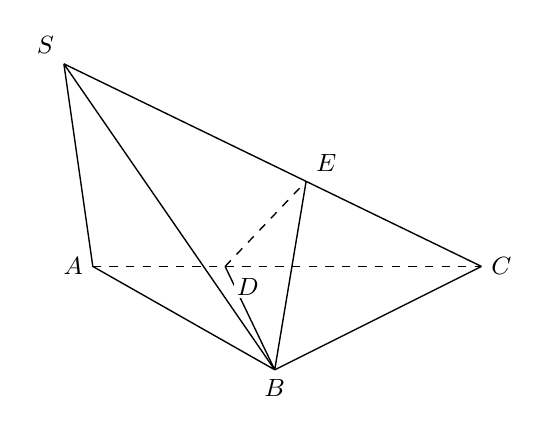
\begin{tikzpicture}[line width=.5pt,scale=1.05,font=\small]
  \coordinate (S) at (1.00,4.15);
  \coordinate (A) at (1.35,1.70);
  \coordinate (C) at (6.05,1.70);
  \coordinate (B) at (3.55,0.45);
  \coordinate (D) at (2.95,1.70);
  \coordinate (E) at (3.93,2.73);
  % 可见棱。
  \draw (S)--(A) (S)--(B) (S)--(C) (A)--(B) (B)--(C);
  % 底面被遮挡的棱 AC，以及截面内的 DE。
  \draw[dashed] (A)--(C);
  \draw[dashed] (D)--(E);
  % 截面 BDE 与底面的交线 BD、截面与面 SBC 的交线 BE。
  \draw (B)--(D) (B)--(E);
  \node[above left] at (S) {$S$};
  \node[left] at (A) {$A$};
  \node[below] at (B) {$B$};
  \node[right] at (C) {$C$};
  \node[fill=white,inner sep=1pt,below right=3pt] at (D) {$D$};
  \node[above right] at (E) {$E$};
\end{tikzpicture}
\end{center}
\nopagebreak[4]
\end{question}
\begin{question}
\gkti{29}（本题满分 14 分）

已知椭圆的焦点为 $F_1(-1,0)$ 和 $F_2(1,0)$，直线 $x=4$ 是椭圆的一条准线。

（1）求椭圆的方程；

（2）又设点 $P$ 在椭圆上，且 $|PF_1|-|PF_2|=1$，求 $\cos\angle F_1PF_2$ 的值。

（源疑点：卷面此式两端的绝对值符号磨损，仅有单竖线，按所见录为 $|PF_1|-|PF_2|=1$；无论是否取外绝对值，本题所求余弦值不变。）

\end{question}
\begin{question}
\gkti{30}（本题满分 14 分）

已知数列 $\{a_n\}$ 的前 $n$ 项和的公式 $S_n=\dfrac{\pi}{12}(2n^2+n)$。

（1）求证 $\{a_n\}$ 是等差数列，并求出它的首项和公差；

\Needspace{5\baselineskip}
（2）记 $b_n=\sin a_n\cdot\sin a_{n+1}\cdot\sin a_{n+2}$，求证：对任何自然数 $n$，都有

\nopagebreak[4]
\[
b_n=\frac{\sqrt2}{8}(-1)^{n-1}.
\]

（源疑点：卷面「并求出它的首项的公差」中「的」字疑为「和」之误，此处按文意录为「首项和公差」。）

\end{question}